% No specific requirements
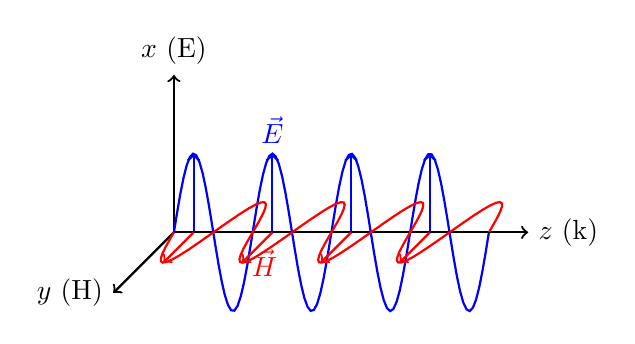
\begin{tikzpicture}
  % Axes
  \draw[->, thick] (0,0,0) -- (4.5,0,0) node[right] {$z$ (k)};
  \draw[->, thick] (0,0,0) -- (0,2,0) node[above] {$x$ (E)};
  \draw[->, thick] (0,0,0) -- (0,0,2) node[left] {$y$ (H)};

  % E-Field (Blue, Vertical)
  \draw[blue, thick, samples=100, domain=0:4] plot (\x, {sin(\x*360)}, 0);
  % H-Field (Red, Horizontal)
  \draw[red, thick, samples=100, domain=0:4] plot (\x, 0, {sin(\x*360)});

  % Vectors at peaks
  \foreach \x in {0.25, 1.25, 2.25, 3.25} {
    \draw[->, blue, thick] (\x,0,0) -- (\x, {sin(\x*360)}, 0);
    \draw[->, red, thick] (\x,0,0) -- (\x, 0, {sin(\x*360)});
  }
  \node[blue, above] at (1.25, 1, 0) {$\vec{E}$};
  \node[red, right] at (1.25, 0, 1) {$\vec{H}$};
\end{tikzpicture}
